\chapter{Результаты}

Все численные методы были реализован в виде программ на языке C++ с использованием библиотеки CUDA \cite{cuda2015} для организации вычислений на графических процессорах. Использовались трехмерные сетки, сгенерированные программой NETGEN v4.9.14 \cite{Netgen2009}.
Для визуализации результатов применялась программа ParaView \cite{Paraview2004}.

\section{Исследование сходимости метода, основанного на вариационном принципе}

Тесты сходимости проводились на задаче об излучении оптически плотного излучающего шара радиуса $R = 0.3$ в поглощающей оптически менее плотной среде (см. приложение \ref{chap:problem}). Сравнивалась плотность энергии излучения. В окрестности поверхности шара плотность энергии имеет логарифмическую особенность производной, такую же, как и в задаче Милна (задача об излучении из полупространства).

Изучалась ошибка в точке $A(0, 0, 0)$ --- центре шара, $B\left(\frac{R}{\sqrt{3}}, \frac{R}{\sqrt{3}}, \frac{R}{\sqrt{3}}\right)$ --- точке на границе шара и в дискретной норме $L_2$:
\[
||u||_{DL_2} = \sqrt{\frac{1}{N}\sum_{i=1}^N u_i^2}
\]

Использовались пространственные сетки с количеством узлов от $7 \cdot 10^3$ до $206 \cdot 10^3$. Для метода сферических гармоник использовались сферические функции до $12$-й степени. Для метода радиальных базисных функций использовались $7$ первых квадратурных формул Лебедева в качестве сетки направлений. 

\subsection{Сходимость методов по количеству угловых функциях}

Анализ сходимости в дискретной норме $L_2$ показал, что зависимость ошибки на самой подробной сетке ($206 \cdot 10^3$ узлов) от числа используемых угловых функций $K$ носит одинаковый характер $\varepsilon \sim K^{-0.29}$, причем ошибка обоих методов практически одинакова при одинаковом количестве используемых угловых функций, см. график на рисунке \ref{fig:UL2err}.

\begin{figure}[ht!]
\centering
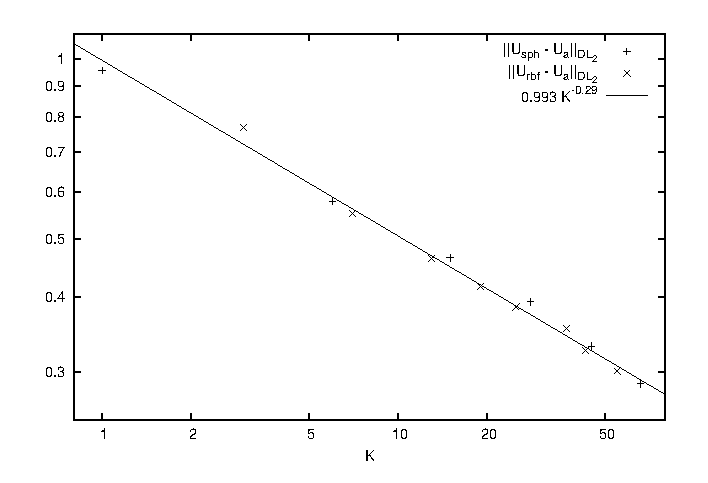
\includegraphics[width=\textwidth]{UL2err.eps}
\caption{Ошибка в норме $||\cdot||_{DL_2}$ в зависимости от числа угловых функций $K$}
\label{fig:UL2err}
\end{figure}

\subsection{Пространственная сходимость методов}

Сходимость методов изучалась в точке $A$ из области гладкости и в точке $B$ с границы шара при использовании самой подробной угловой дискретизации. Сходимость изучалась в зависимости от характерного шага сетки, принятого равным $N^{-1/3}$. На рисунке \ref{fig:UAerr} изображены графики ошибки в области гладкости и на границе шара.

\begin{figure}[ht!]
\centering
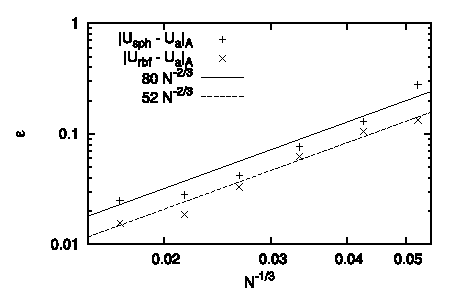
\includegraphics[width=.49\textwidth]{UAerr.eps}
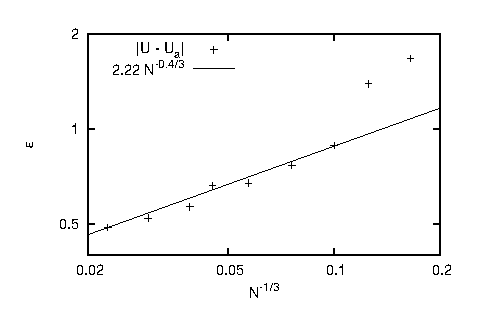
\includegraphics[width=.49\textwidth]{UBerr.eps}
\caption{Ошибка в точках $A, B$ в зависимости от характерного шага сетки $N^{-1/3}$}
\label{fig:UAerr}
\end{figure}

Порядок сходимости обоих методов в области гладкости равен двум. В области шара, где коэффициент поглощения меняется скачкообразно, порядок сходимости разный, он равен $\sim 0.4$ для метода сферических гармоник и $\sim 0.3$ для метода с радиальными базисными функциями, хотя разброс данных не позволяет достоверно определить порядок сходимости.

На рисунке \ref{fig:anvsnum} представлено решения вдоль оси $Ox$, полученные методом с радиальными функциями при $K = 55$ и методом сферических гармоник при $K = 91$. Видно, что существенное отличие численного решения от аналитического наблюдается в поглощающей области в окрестности шара.

Для обоих методов свойственны нефизичные значения интенсивности в области вдали от шара. Функция интенсивности, восстановленная из гармоник решения
\[
I(\vec r, \vec \Omega) = \sum_{k=1}^{n} I_k(\vec r) \theta_k (\vec \Omega)
\]
может содержать значения с отрицательными значениями интенсивности. В случае $I(\vec r, \vec \Omega) > 0$ тензор направленности излучения (тензор квазидиффузии) $\mathbb D$, определяемый как
\[
\mathbb D = \frac{\mathbb T}{U} = \frac{\int_{4\pi} \vec \Omega\vec \Omega I(\vec r, \vec \Omega) d\Omega}{\int_{4\pi} I(\vec r, \vec \Omega) d\Omega}
\]
имеет след, равный $1$ и неотрицательные компоненты. Однако, в численных расчетах свойство неотрицательности может нарушаться, если интенсивность $I(\vec r, \vec \Omega)$ принимает отрицательные значения (см. график на рисунке \ref{fig:Drad}). Значения $D_{rr} > 1$ свидетельствуют об отрицательности двух других главных компонент тензора $\mathbb D$.

\begin{figure}[ht!]
\centering
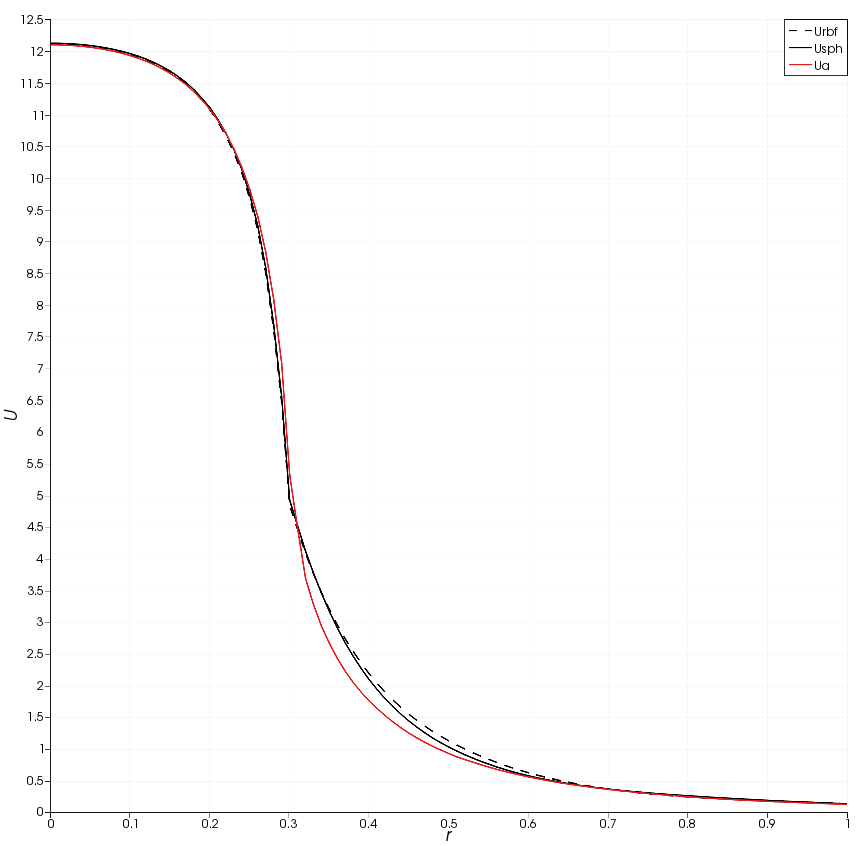
\includegraphics[width=.5\textwidth]{Uanvsnum.png}
\caption{Решения вдоль оси $Ox$, полученные методом с радиальными функциями при $K=55$ и методом сферических гармоник при $K = 91$}
\label{fig:anvsnum}
\end{figure}

\begin{figure}[ht!]
\centering
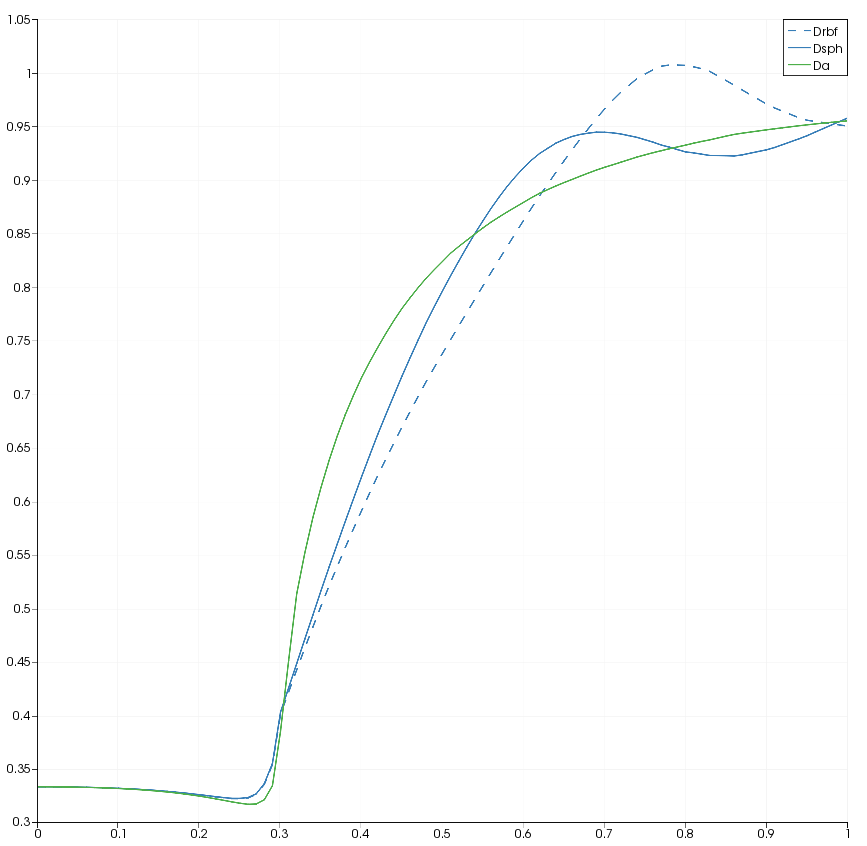
\includegraphics[width=.5\textwidth]{Dxx.png}
\caption{Радиальная компонента тензора направленноcти $\mathbb D_{rr}$ вдоль оси $Ox$}
\label{fig:Drad}
\end{figure}

Для исследования эффекта луча рассмотрим изоповерхности плотности интенсивности. Для метода сферических гармоник эффект луча отсутствует, поскольку базис из сферических функций инвариантен относительно произвольных вращений. На рисунке \ref{fig:iso} изображены изоповерхности решения построены для случая $K = 15$ метода сферических гармоник и $K = 13$ метода с радиальными функциями.

\begin{figure}[ht!]
\centering
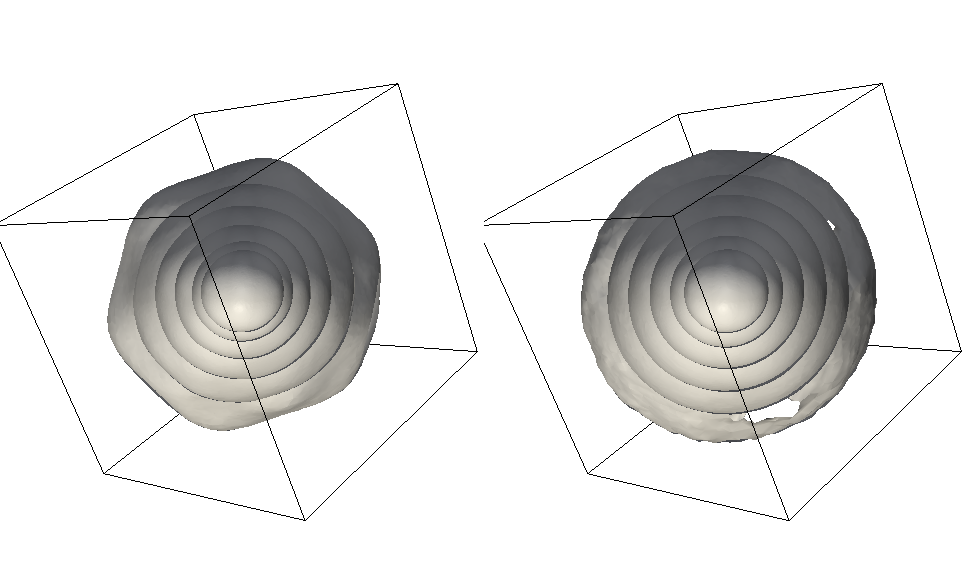
\includegraphics[width=\textwidth]{iso.png}
\caption{Изоповерхности плотности энергии излучения для метода с радиальными функциями (слева) и сферическими гармониками (справа)}
\label{fig:iso}
\end{figure}

\subsection{Сходимость метода при использовании предобуславливателя}

Для исследования сходимости внешних итераций метода сопряженных градиентов изучалось количество вызовов предобуславливателя для уменьшения нормы невязки в $10^{6}$ раз.

Отметим, что для метода сопряженных градиентов число итераций увеличивается как с увеличением количества угловых гармоник $K$, так и увеличением количества узлов сетки $N$. Для метода с радиальным базисом число итераций практически постоянно и равно $30$.

\begin{table}[ht!]
\RawFloats
\centering
\caption{Количество итераций метода сопряженных градиентов}
\begin{tabular}{cc|c|c|c|c|c|c|}
\cline{3-8}
& & \multicolumn{6}{|c|}{\rule{0em}{2.2ex}Количество узлов сетки} \\ \cline{3-8}
& & \rule{0em}{2.2ex}6996 & 12971 & 26786 & 53109 & 99015 & 205756\\ \cline{1-8}
\multicolumn{1}{|c|}{\multirow{7}{*}{\rotatebox{90}{Угловых  гармоник\phantom{x}}}} &
\multicolumn{1}{|c|}{\rule{0em}{2.2ex}1}  & 1 & 1 & 1 & 1 & 1 & 1 \\ 
\cline{2-8}\multicolumn{1}{|c|}{} &
\multicolumn{1}{|c|}{\rule{0em}{2.2ex}6}  & 20 & 21 & 22 & 23 & 25 & 26 \\ 
\cline{2-8}\multicolumn{1}{|c|}{} &
\multicolumn{1}{|c|}{\rule{0em}{2.2ex}15} & 29 & 31 & 33 & 34 & 37 & 38 \\ 
\cline{2-8}\multicolumn{1}{|c|}{} &
\multicolumn{1}{|c|}{\rule{0em}{2.2ex}28} & 36 & 38 & 41 & 44 & 48 & 51 \\ 
\cline{2-8}\multicolumn{1}{|c|}{} &
\multicolumn{1}{|c|}{\rule{0em}{2.2ex}45} & 42 & 45 & 49 & 53 & 57 & 62 \\ 
\cline{2-8}\multicolumn{1}{|c|}{} &
\multicolumn{1}{|c|}{\rule{0em}{2.2ex}66} & 46 & 50 & 55 & 60 & 65 & 70 \\ 
\cline{2-8}\multicolumn{1}{|c|}{} &
\multicolumn{1}{|c|}{\rule{0em}{2.2ex}91} & 48 & 53 & 59 & 65 & 71 & 77 \\ 
\cline{1-8}
\end{tabular}
\end{table}

\begin{table}[ht!]
\RawFloats
\centering
\caption{Количество итераций метода с радиальным базисом}
\begin{tabular}{cc|c|c|c|c|c|c|}
\cline{3-8}
& & \multicolumn{6}{|c|}{\rule{0em}{2.2ex}Количество узлов сетки} \\ \cline{3-8}
& & \rule{0em}{2.2ex}6996 & 12971 & 26786 & 53109 & 99015 & 205756\\ \cline{1-8}
\multicolumn{1}{|c|}{\multirow{7}{*}{\rotatebox{90}{Угловых гармоник\phantom{x}}}} &
\multicolumn{1}{|c|}{\rule{0em}{2.2ex}3}  & 13 & 14 & 15 & 14 & 15 & 15 \\ 
\cline{2-8}\multicolumn{1}{|c|}{} &
\multicolumn{1}{|c|}{\rule{0em}{2.2ex}7}  & 26 & 27 & 28 & 28 & 29 & 31 \\ 
\cline{2-8}\multicolumn{1}{|c|}{} &
\multicolumn{1}{|c|}{\rule{0em}{2.2ex}13} & 33 & 34 & 35 & 36 & 39 & 42 \\ 
\cline{2-8}\multicolumn{1}{|c|}{} &
\multicolumn{1}{|c|}{\rule{0em}{2.2ex}19} & 26 & 28 & 29 & 29 & 30 & 32 \\ 
\cline{2-8}\multicolumn{1}{|c|}{} &
\multicolumn{1}{|c|}{\rule{0em}{2.2ex}25} & 28 & 29 & 32 & 30 & 32 & 34 \\ 
\cline{2-8}\multicolumn{1}{|c|}{} &
\multicolumn{1}{|c|}{\rule{0em}{2.2ex}43} & 28 & 30 & 32 & 31 & 33 & 34 \\ 
\cline{2-8}\multicolumn{1}{|c|}{} &
\multicolumn{1}{|c|}{\rule{0em}{2.2ex}55} & 27 & 28 & 30 & 29 & 30 & 32 \\ 
\cline{1-8}
\end{tabular}
\end{table}

\section{Исследование маршевого метода коротких характеристик}

Для метода коротких характеристик изучалась численная диффузия луча. Центральное излучательное тело было заменено на крест, составленный из пяти одинаковых кубов (см. рисунок \ref{fig:cross}). Решение строилось для одного направления, при этом аналитическое решение представляет собой проекцию креста на грань тетраэдра. Оптическая толщина креста много больше единицы, а оптическая толщина окружающего пространства много меньше единицы. В таких условиях, решение на грани имеет интенсивность равную равновесной интенсивности в кресте.
\begin{figure}[ht!]
\centering
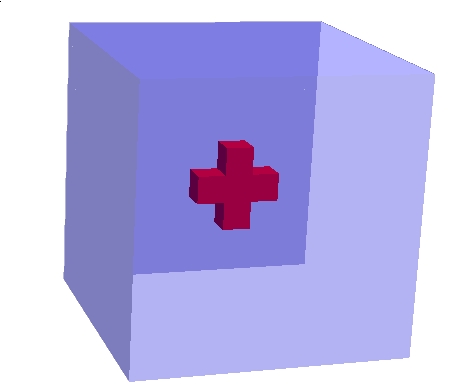
\includegraphics[width=.5\textwidth]{plus.png}
\caption{Вид излучающего тела для метода коротких характеристик}
\label{fig:cross}
\end{figure}

%\subsection{Сравнение численной диффузии луча в методах первого и второго порядка}

Для метода первого порядка решение на грани испытывает значительную диффузию. Для метода второго порядка без ограничителя решение нарушает принцип максимума. Отклонения интенсивности на грани от диапазона $[0, 1]$ составляет $20 \%$ (области на границе креста). Метод с ограничителем имеет решение, в котором принцип максимума не нарушен, а численная диффузия луча значительно меньше, чем в случае метода первого порядка.

\begin{figure}[ht!]
\centering
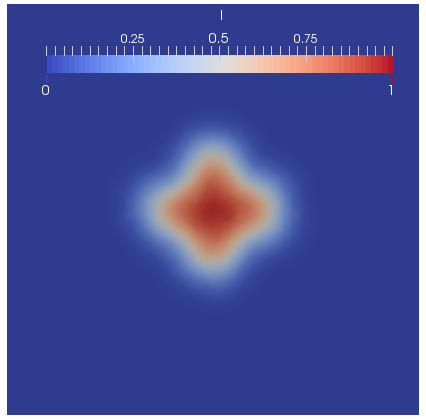
\includegraphics[width=.3\textwidth]{res1ord.png}
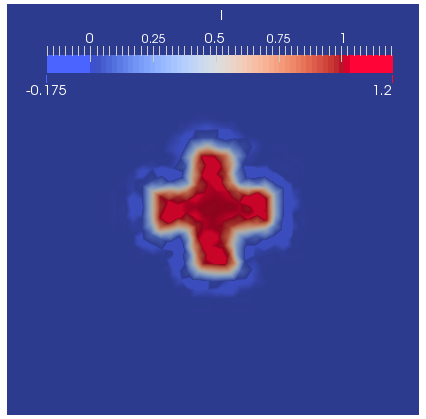
\includegraphics[width=.3\textwidth]{res2nolim.png}
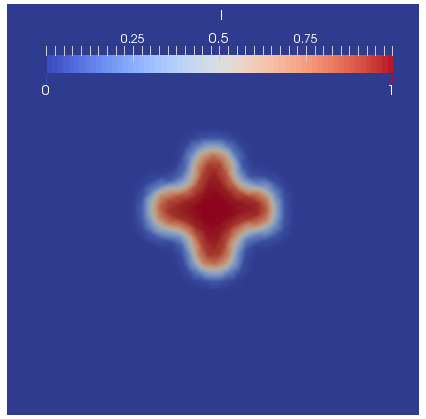
\includegraphics[width=.3\textwidth]{res2wilim.png}
\caption{Решение на грани для метода первого порядка (слева), метода второго порядка (в центре) и метода второго порядка с ограничителем (справа)}
\label{fig:limiter}
\end{figure}

Сравнение плотности излучения в решениях, полученных методом первого и второго порядка с ограничителем показывает близкие (в пределах $2\%$) решения (см графики на рисунках \ref{fig:U2vs1} и \ref{fig:U2vs1Line}). При этом для метода второго порядка плотность энергии излучения сосредоточена в кресте, в то время как в методе первого порядка она диффундирует за его пределы. К тому же, в методе второго порядка более выражен эффект луча, в методе же первого порядка, он сглажен численной диффузией.

\begin{figure}[ht!]
\centering
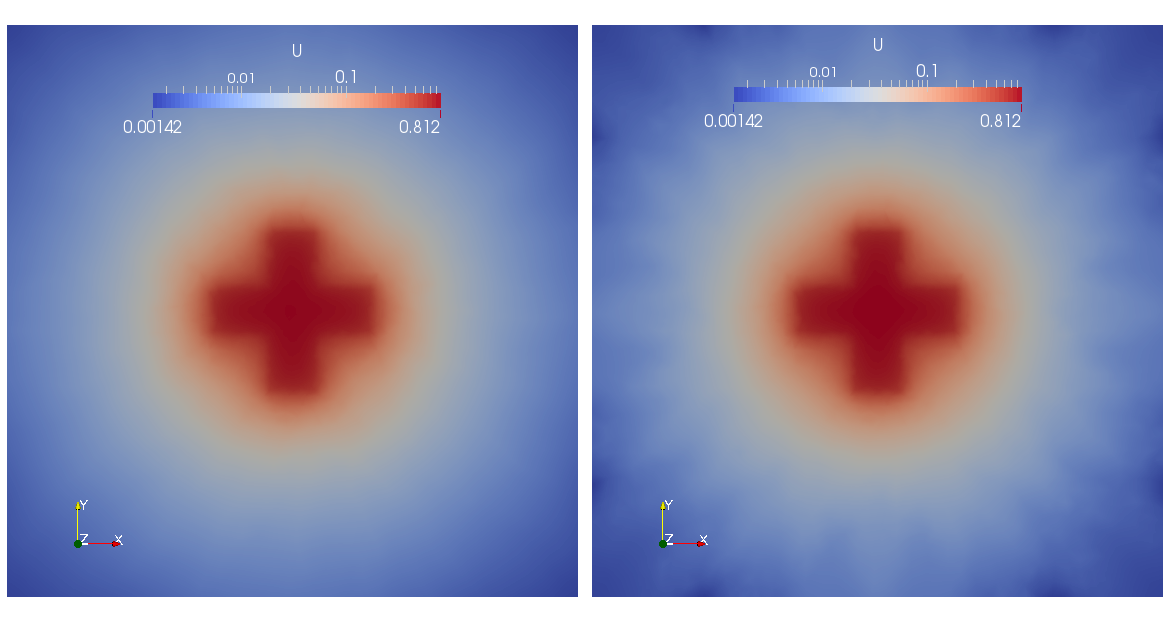
\includegraphics[height=.3\textheight]{U2vs1.png}
\caption{Плотность излучения в методе первого порядка (слева) и второго порядка с ограничителем (справа) в центральном сечении}
\label{fig:U2vs1}
\end{figure}

\begin{figure}[ht!]
\centering
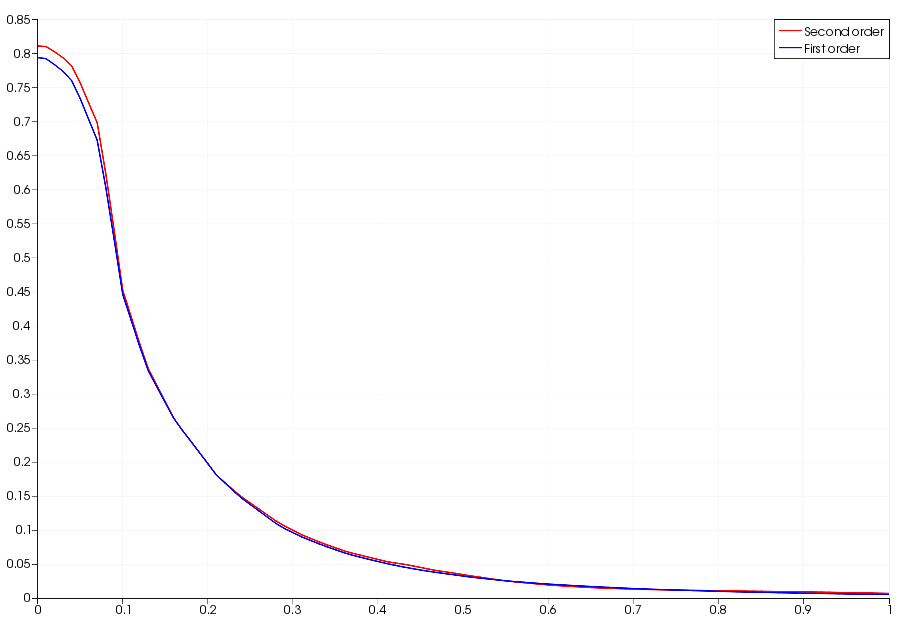
\includegraphics[height=.3\textheight]{U2vs1Line.png}
\caption{Плотность излучения в методе первого порядка (синий график) и второго порядка с ограничителем (красный график) вдоль луча, перпендикулярного кресту}
\label{fig:U2vs1Line}
\end{figure}

Дополнительно был рассмотрен метод первого порядка с увеличенным количеством узлов. В этом методе вместо квадратичной интерполяции по шести узлам используется кусочно-линейная. Данная операция позволяет сравнивать методы при одинаковом числе используемых узлов. Область и излучающее тело были заменены на концентрические шары, а поглощение в области отсутствовало. Диффузия луча носит качественно различный характер: в методе первого порядка диффузия луча имеет характер $\sim \sqrt{x}$, а в методе второго порядка диффузия луча практически постоянна вдоль луча.

\begin{figure}[ht!]
\centering
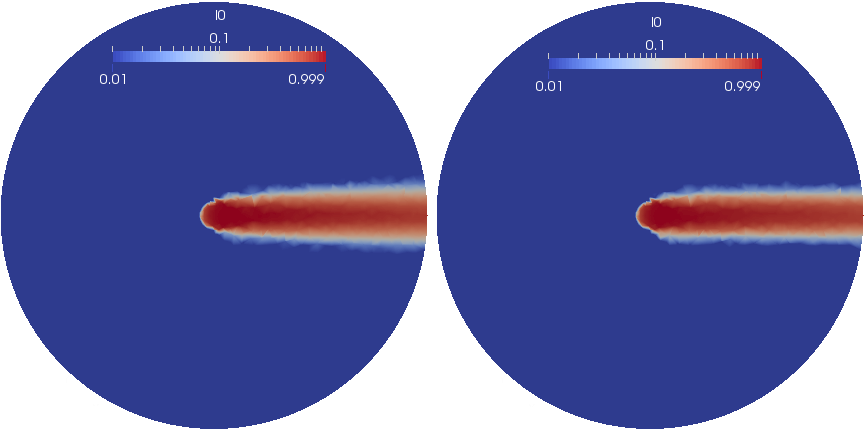
\includegraphics[width=\textwidth]{diff.png}
\caption{Диффузия луча в методе первого порядка с увеличенным числом узлов (слева) и методе второго порядка с ограничителем}
\label{fig:diff}
\end{figure}

\section{Исследование распределенного метода длинных характеристик}

\subsection{Сравнение решений для различного числа подобластей}

Для нескольких подобластей наблюдается незначительная диффузия луча, проходящего через границу подобластей.

\subsection{Ускорение и эффективность параллельной реализации}

Версия, использующая графические ускорители в $3.5$ раз быстрее версии для центрального процессора.

\section{Расчет спектра излучения линии H-$\alpha$ звезды типа Т Тельца}

\section{Выводы}
